\documentclass[12pt]{article}
\usepackage{../gongkechuang}

\title{EI313-DPDK \texttt{l2fwd} Performance Test}

\begin{document}

\maketitle

In this report, the performance of L2-forwarding on virtual machines, implemented with \emph{Data Plane Development Kit}, are tested.

\section{Introduction}

DPDK provides a high-throughput design on data processing on Linux, replacing the kernel design. For \texttt{l2fwd}, it utilizes multiple memory tricks, and forwarding the packet in the driver state, without sending it to kernel, which will boost the network performance.

\section{Experiment Environment Configuration}

\subsection{Compile \texttt{DPDK} and Test Utility}

The DPDK package provided by Arch Linux uses newer CPU which has instruction set that our CPU, namely Haswell structure, does not support. We modified the build script to support them.

Compared to the official documentation \emph{getting started with \texttt{pktgen}}, which uses environmental variables to specify the compiling configuration, the newer version, in our example 21.11, uses \texttt{meson} to configure automatically and \texttt{ninja}, a UNIX \texttt{make} alternative, to build and install them.

\begin{lstlisting}[caption={Build Script of \texttt{dpdk}}]
pkgname=dpdk-haswell

...

build() {
  cp -r dpdk-$pkgver dpdk-orig
  cd dpdk-orig
  meson build --prefix=/usr
  ninja -C build
}

package () {
    cd dpdk-orig
    DESTDIR="$pkgdir" ninja -C build install
}

\end{lstlisting}

\begin{lstlisting}[caption={Build Script of \texttt{dpdk-utils}}]
pkgbase=dpdk-utils
pkgname=( dpdk-helloworld dpdk-l2fwd  )

...

build_helloworld () {
    cd dpdk-$pkgver/examples/helloworld
    make
}

build_l2fwd () {
    cd dpdk-$pkgver/examples/l2fwd
    make
}



build() {
  (build_helloworld)
  (build_l2fwd)
}

package_dpdk-helloworld () {
    depends+=(dpdk-haswell)
    cd dpdk-$pkgver/examples/helloworld
    install -Dm755 build/helloworld $pkgdir/usr/bin/dpdk-helloworld
}

package_dpdk-l2fwd () {
    depends+=(dpdk-haswell)
    cd dpdk-$pkgver/examples/l2fwd
    install -Dm755 build/l2fwd $pkgdir/usr/bin/dpdk-l2fwd
}

\end{lstlisting}

\begin{lstlisting}[caption={Build Script of \texttt{dpdk-pktgen}}]
pkgname=dpdk-pktgen
pkgver=21.11

...

build() {
    cd pktgen-dpdk-pktgen-$pkgver.$pkgrel
    meson build --prefix=/usr
    ninja -C build
}

package () {
    cd pktgen-dpdk-pktgen-$pkgver.$pkgrel
    DESTDIR="$pkgdir" ninja -C build install
}
\end{lstlisting}

To provide virtio support, we compiled the packages on a building VM.

\subsection{Virtual Machine Configuration}

The virtual machine running \texttt{l2fwd} is configured with 2 CPU and 2GB memory, with 512$\times$2MB$=$1GB huge pages. The virtual machine running \texttt{pktgen} is configured with 2 CPU and 4GB memory, with 1536$\times$2MB$=$3GB huge pages. As our DPDK packages are build and configured supporting the host CPU, we need to set the VM to copy the configuration of host CPU. The libvirt XML configuration shows the details:

\begin{lstlisting}[language=xml]
  <cpu mode="host-passthrough" check="partial" migratable="on"/>
\end{lstlisting}

\texttt{DPDK} also utilizes hugepages to perform, so we need to modify VM's hugepage configuration. The configuration script to install all dependencies, modify hugepage configurations. VM running it is shown in figure \ref{fig:config-vm}.


\begin{lstlisting}[caption={Contents of \texttt{configure\_hugepage.sh}}]
#!/bin/bash

echo 'Server = https://mirror.sjtu.edu.cn/archlinux/$repo/os/$arch' > /tmp/$$-ml
sudo cp /tmp/$$-ml /etc/pacman.d/mirrorlist

sudo pacman --noconfirm -Syu
sudo pacman --noconfirm -U ./*.tar.zst

sudo sed -i "s/ifnames=0\"/ifnames=0 \
default_hugepagesz=2M hugepagesz=2M hugepages=512  transparent_hugepage=never\"/g" /etc/default/grub

# Huge pages on pktgen is 1536.

sudo grub-mkconfig -o /boot/grub/grub.cfg

sudo shutdown now
\end{lstlisting}

All VMs has 3 NICs configured to it. The first one is used for Internet connection, and the second one, connected to the same virtual switch of NIC 1, is set as port 0 in DPDK function series. We created another virtual switch, where NIC 2 is connected to, and set as port 1 in DPDK function series. The network topology are shown as figure \ref{fig:net_topo}.

\begin{figure}[ht]
    \centering
    \def\svgwidth{0.3\textwidth}
    \tiny
    \input{figures/connection.pdf_tex}
    \caption{Network Topology}
    \label{fig:net_topo}
\end{figure}

\subsection{Network Configuration}

The port using by DPDK needs to be load with special drivers and binded. For the link that we want to bind to DPDK, for example, eth0, we need to set it down:

\begin{lstlisting}
sudo ip link set dev eth0 down
\end{lstlisting}

As DPDK does not support virtio driver, Then we need to probe a supported driver \texttt{uio\_pci\_generic}:

\begin{lstlisting}
sudo modprobe uio_pci_generic
\end{lstlisting}

Then we use \texttt{dpdk-devbind.py} to bind it to the device.

\begin{lstlisting}
sudo dpdk-devbind.py -b uio_pci_generic eth0
\end{lstlisting}

The procedures are shown in figure \ref{fig:bind}. We also writes a script to bind eth1 and eth2 automatically.

\begin{lstlisting}[caption={bind\_port.sh}]
#!/bin/bash

sudo ip link set dev eth1 down
sudo ip link set dev eth2 down
sudo modprobe uio_pci_generic
sudo dpdk-devbind.py -b uio_pci_generic eth1
sudo dpdk-devbind.py -b uio_pci_generic eth2
\end{lstlisting}

\section{Performance Test}

\subsection{Configure \texttt{pktgen}}

\texttt{pktgen} is a tool that sends and receives package, recording its performance with DPDK infrastructure. First we starts the \texttt{pktgen}.

\begin{lstlisting}
sudo pktgen -l 0-1 -n 2 -- -P -m "[1].0,[1].1"
\end{lstlisting}

The parameters:

\begin{itemize}
    \item EAL part
    \begin{itemize}
        \item \texttt{-l 0-1} Uses core 0 and core 1, as \texttt{pktgen} requested.
        \item \texttt{-n 2} Use 2 memory channels.
    \end{itemize}
    \item \texttt{pktgen} part
    \begin{itemize}
        \item \texttt{-P} Enable promiscuous mode
        \item \texttt{ -m "[1].0,[1].1"} Use logical core 1 to process both port 0 and 1's receiving and transmitting.
    \end{itemize}
\end{itemize}

The \texttt{pktgen} is defaulted to appoint the neighbour port as the receiver. In the \texttt{pktgen} CLI, we start the transmission by running:

\begin{lstlisting}
Pktgen:/> start 0
\end{lstlisting}

As shown in the figure \ref{fig:pktgen}, the port 2, marked red, starts to send out packages. However, as port 2 and port 3 are not in the same sub-network, the packet will not reach port 3.

\begin{figure}[ht]
    \centering
    \def\svgwidth{0.3\textwidth}
    \tiny
    \input{figures/pktgen.pdf_tex}
    
    Red: Port 0, Green Port 1
    \caption{\texttt{pktgen} Configuration}
    \label{fig:pktgen}
\end{figure}

We could see from figure \ref{fig:pktgen-no-l2fwd}, that the TX rate is 157MBits/s, while port 1 has no RX.


\subsection{Configure \texttt{l2fwd}}

The \texttt{l2fwd} provided by DPDK is designed to forward packets to neighbour ports. We first stop the \texttt{pktgen} transmission we started above, and start the \texttt{l2fwd}:

On \texttt{pktgen} VM:
\begin{lstlisting}
Pktgen:/> stop 0
\end{lstlisting}

On \texttt{l2fwd} VM:
\begin{lstlisting}
sudo dpdk-l2fwd -c 0x1 -n 4 -- -p 0x3 -q 2
\end{lstlisting}

The parameters:

\begin{itemize}
    \item EAL part
    \begin{itemize}
        \item \texttt{-c 0x1} Uses 1 logical core.
        \item \texttt{-n 4} Use 4 memory channels.
    \end{itemize}
    \item \texttt{l2fwd} part
    \begin{itemize}
        \item \texttt{-p 0x3} Assign DPDK port 0 and 1 (port 2 and 3 as figure).
        \item \texttt{ -q 2} RX/TX queue number per logical core.
    \end{itemize}
\end{itemize}

We could see from figure \ref{fig:l2fwd-no-pktgen}, that there's only around 100 packet maximum transmitted in the network every second.


\subsection{Combining \texttt{l2fwd} and \texttt{pktgen}}

We recover the transmission on the \texttt{pktgen} VM:

\begin{lstlisting}
Pktgen:/> start 0
\end{lstlisting}

Then the transmission is performed as figure \ref{fig:transmission}.

\begin{figure}[ht]
    \centering
    \def\svgwidth{0.3\textwidth}
    \tiny
    \input{figures/l2fwd.pdf_tex}
    \caption{\texttt{l2fwd} forwarding packages}
     \label{fig:transmission}
\end{figure}

We can see from the packet status from both VM, that the packages are forwarded as intended.


\subsection{Analysis}

The \texttt{l2fwd}'s transmission is shown in table \ref{tbl:transmitted} and figure \ref{fig:transmitted}.

\begin{table}[ht]
\caption{Transmitted Packets}\label{tbl:transmitted}
\footnotesize
\centering
\begin{tabular}{c|cccccc}
\hline
Time        & 0       & 10       & 20       & 30       & 40       & 50       \\ \hline
Received    & 0       & 1605515  & 3045976  & 4497626  & 6033029  & 7511865  \\
Transmitted & 0       & 1317195  & 2680740  & 3823783  & 4911358  & 6152288  \\
Rate        & 0       & 22\%     & 14\%     & 18\%     & 23\%     & 22\%     \\ \hline
Time        & 60      & 70       & 80       & 90       & 100      & 110      \\
Received    & 9074176 & 10686744 & 12215089 & 13617841 & 15021751 & 16604369 \\
Transmitted & 7332041 & 8477683  & 9562542  & 10814338 & 11907190 & 12998586 \\
Rate        & 24\%    & 26\%     & 28\%     & 26\%     & 26\%     & 28\%     \\ \hline
\end{tabular}
\end{table}

\begin{figure}[ht]
    \centering
    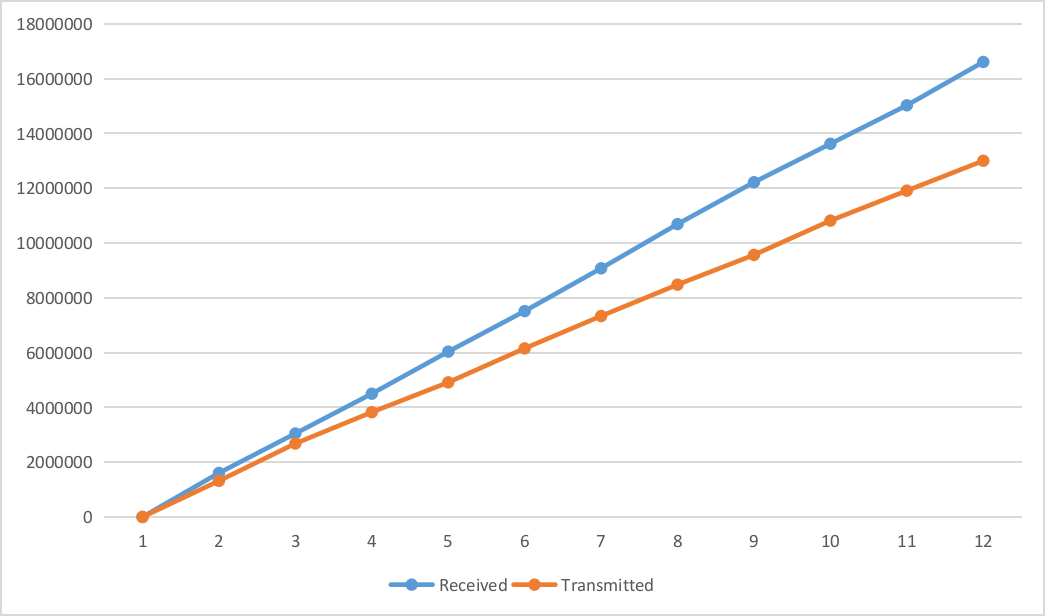
\includegraphics[width=0.85\textwidth]{figures/figure-l2fwd.png}
    \caption{Figure of \texttt{l2fwd} transmitted packets}
    \label{fig:transmitted}
\end{figure}


We could observe that the packets transmitting rate is arount 70MB/s, while receiving rate is around 35MB/s, suffering 50\% loss. The \texttt{l2fwd} module only dropped about 25\% packets. We could infer from the packet dropping rate, and the packets sent and received by \texttt{l2fwd} and \texttt{pktgen}, that the switches forwarding at host machine's linux kernel is causing around 18\% of packet loss each, and 33\% total. 

We observe that with just a single core configuration and 1GB of memory, the loss of \texttt{l2fwd} is already close to the forwarding capacity of the host linux kernel. This loss can be further reduced by increasing the number of operating cores and hugepages of \texttt{l2fwd}.

\section{Conclusion}

\emph{omitted}

\newpage
\section*{Screenshot}

\begin{figure}[ht]
    \centering
    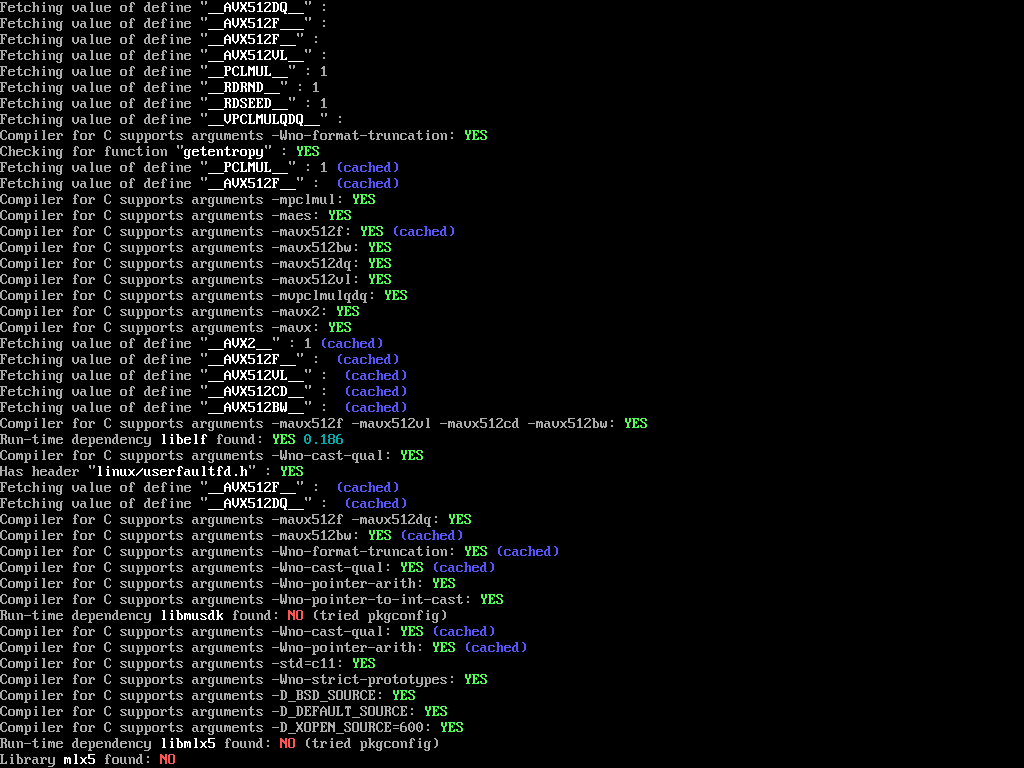
\includegraphics[width=0.7\textwidth]{figures/build-dpdk.png}
    \caption{Build DPDK and Utilities on VM}
    \label{fig:build}
\end{figure}


\begin{figure}[ht]
    \centering
    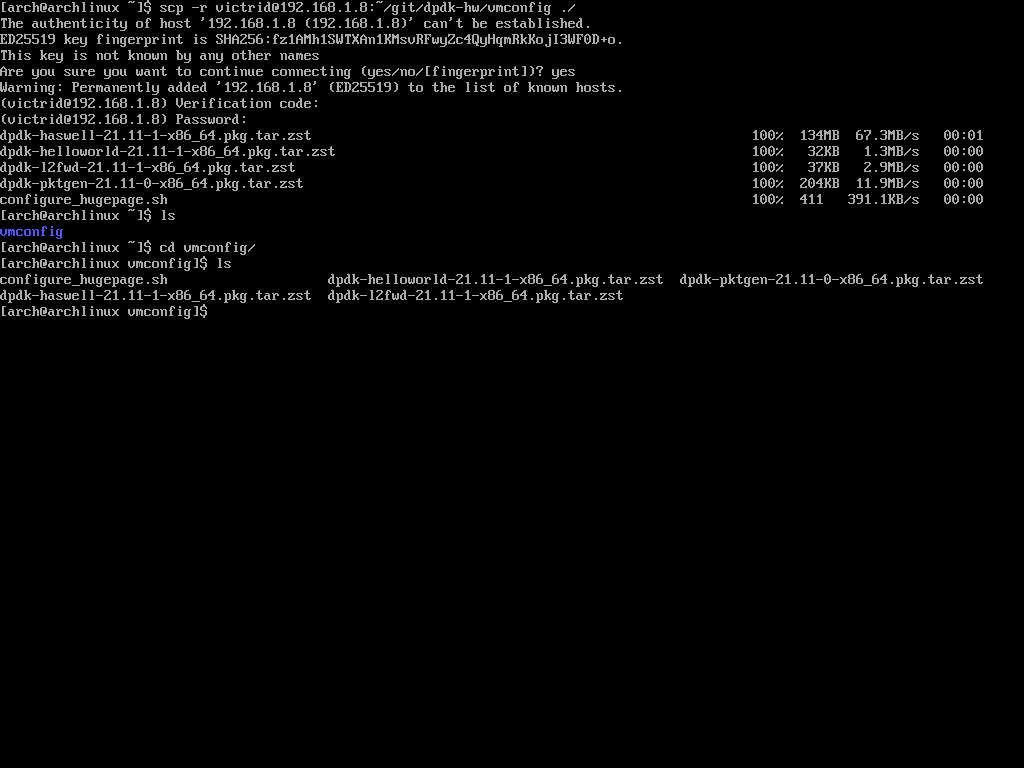
\includegraphics[width=0.7\textwidth]{figures/config-vm.png}
    \caption{VM configuration}
    \label{fig:config-vm}
\end{figure}

\begin{figure}[ht]
    \centering
    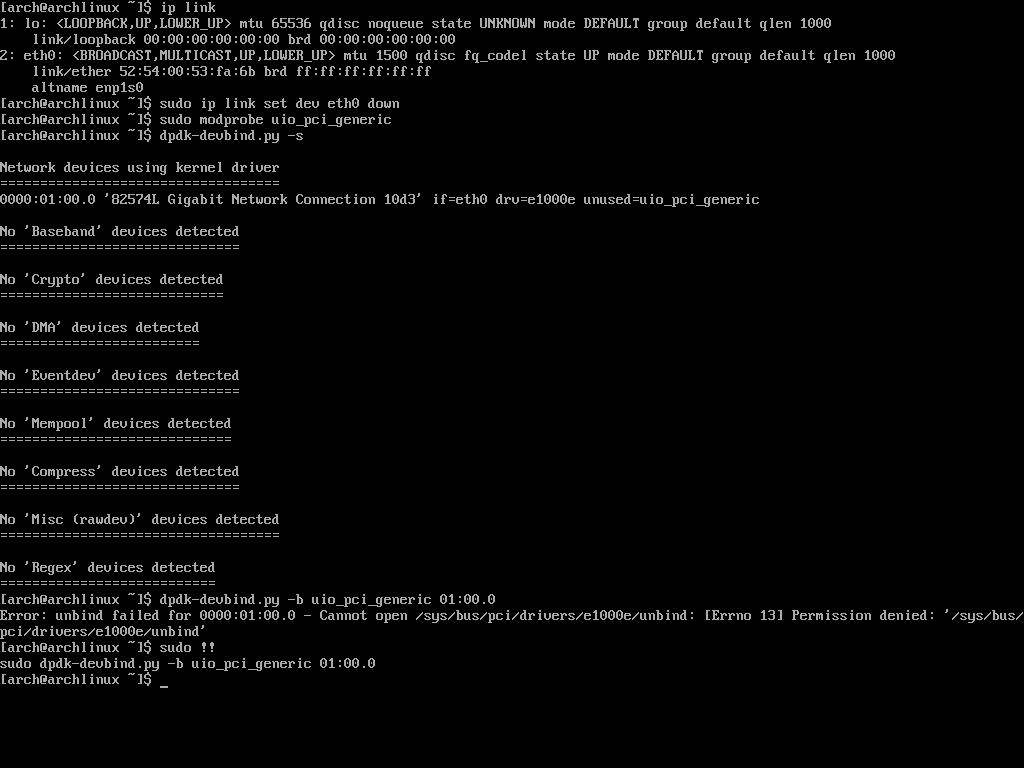
\includegraphics[width=0.7\textwidth]{figures/bind_port.png}
    \caption{Bind the port}
    \label{fig:bind}
\end{figure}

\begin{figure}[ht]
    \centering
    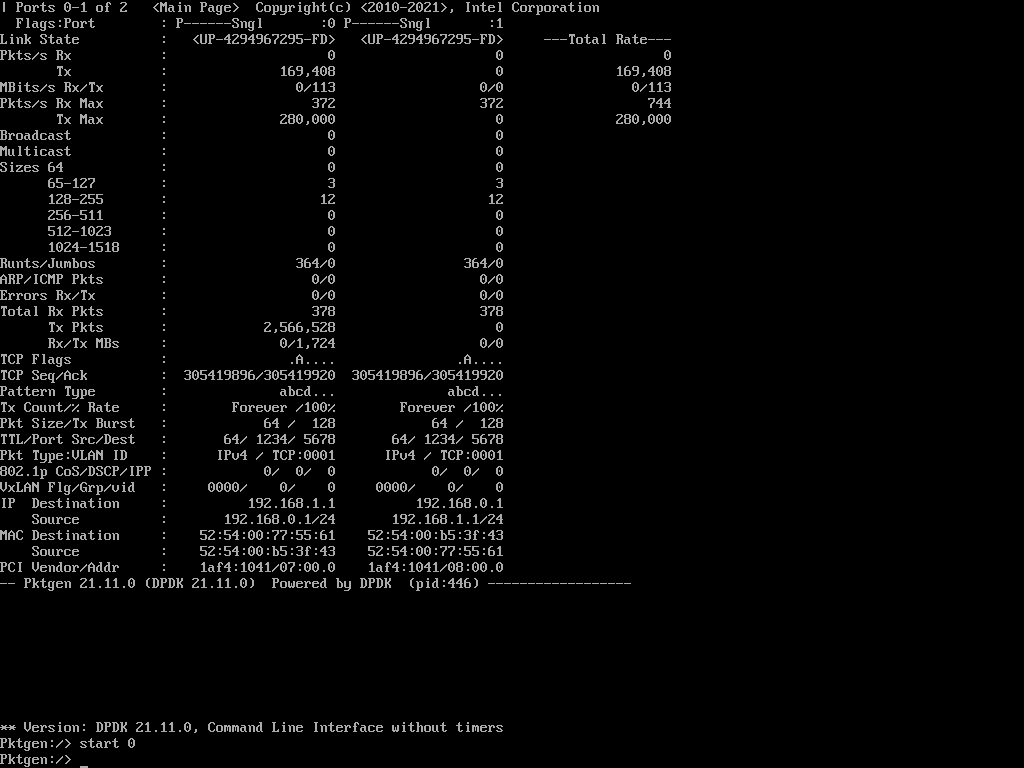
\includegraphics[width=0.7\textwidth]{figures/no-l2fwd.png}
    \caption{\texttt{pktgen} without l2fwd}
    \label{fig:pktgen-no-l2fwd}
\end{figure}

\begin{figure}[ht]
    \centering
    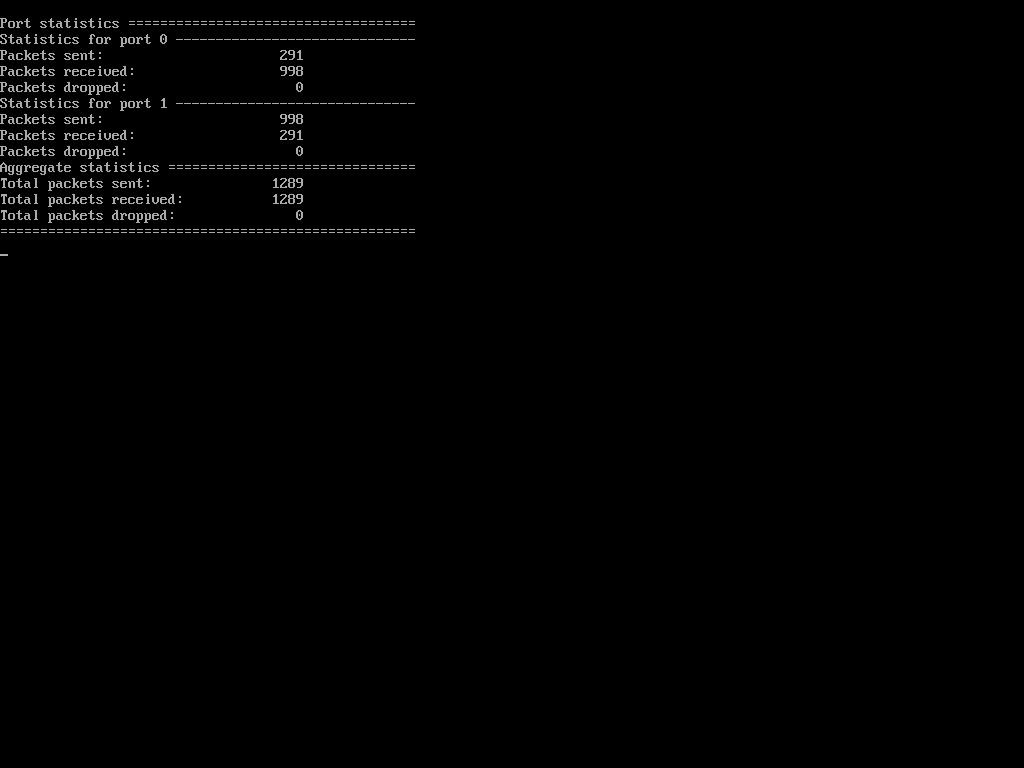
\includegraphics[width=0.7\textwidth]{figures/no-pktgen.png}
    \caption{Running raw l2fwd, first 10s}
    \label{fig:l2fwd-no-pktgen}
\end{figure}


\begin{figure}[ht]
    \centering
    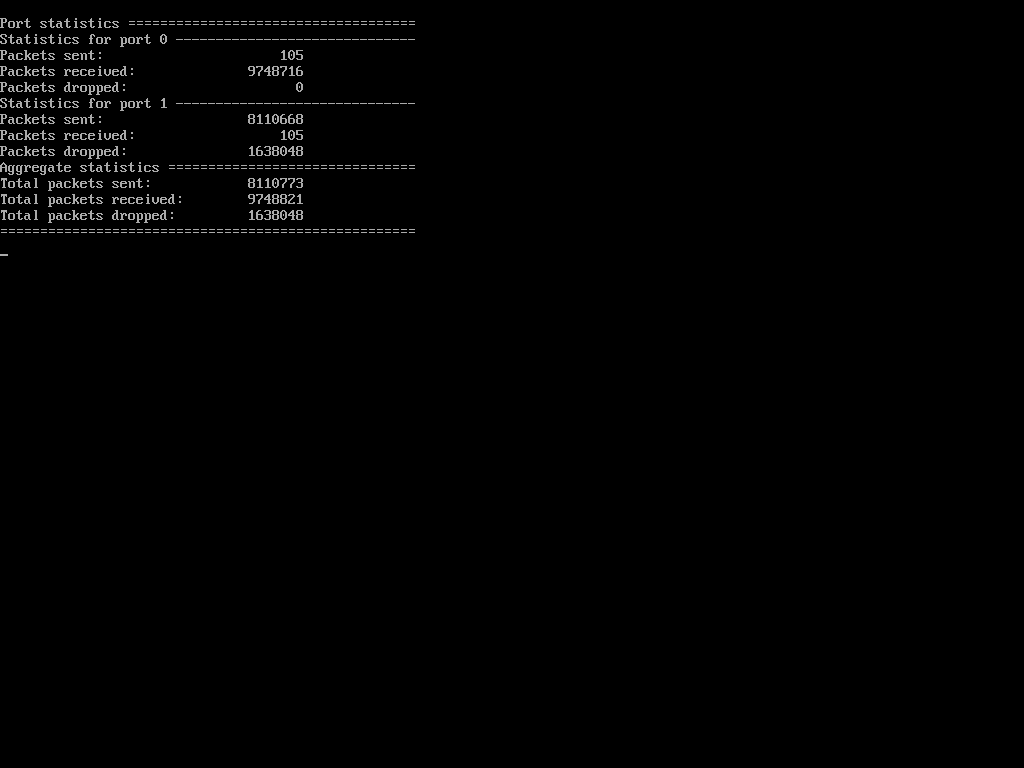
\includegraphics[width=0.7\textwidth]{figures/l2fwding.png}
    
    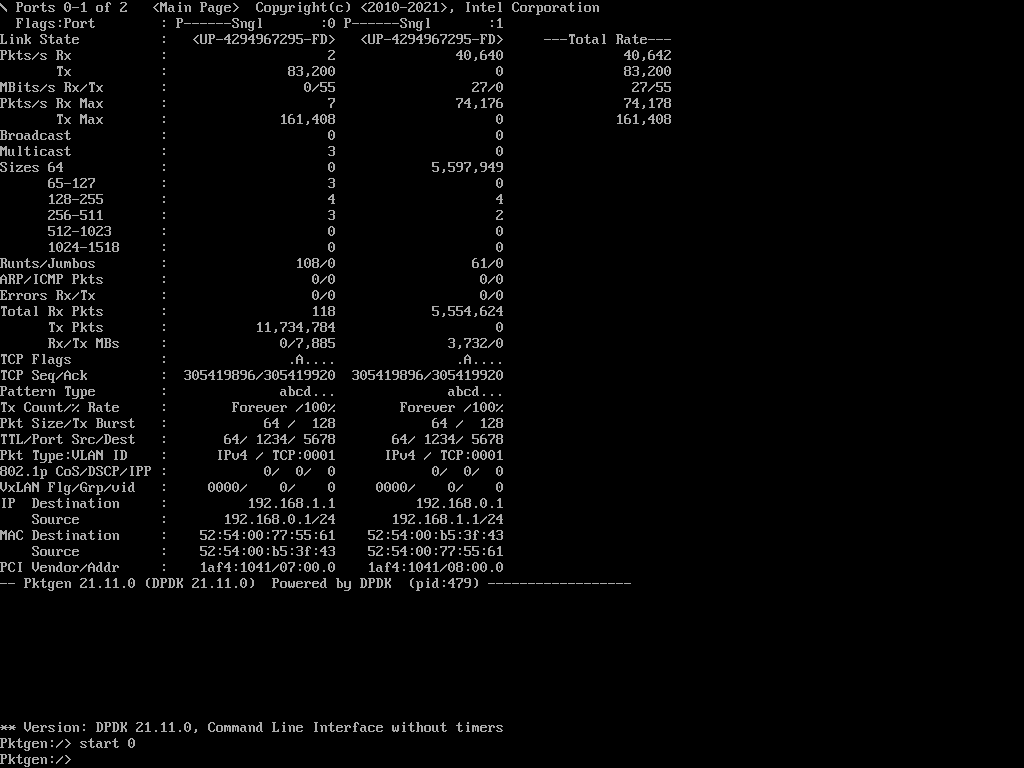
\includegraphics[width=0.7\textwidth]{figures/pktgening.png}
    \caption{Data Rate}
     \label{fig:data}
\end{figure}

\end{document}

